\documentclass[../../Rapport RayTracer]{subfiles}


\begin{document}

Pour calculer un rendu, le RayTracer a besoin de:
\begin{itemize}
	\item{Une résolution de rendu}
	\item{Une scène contenant les objets à rendre}
	\item{Une ou plusieures sources de lumière}
	\item{Une caméra}
	\item{Un nombre de thread sur lequel le rendu sera effectué}
\end{itemize}
La résolution de rendu est fixe et est donnée au constructeur du RayTracer. Les autres réglages, se trouvant dans la classe \textit{RayTracerSettings} sont quant à eux dynamiques. S'ils sont modifiés, le ray tracer adaptera alors son rendu en conséquence et en temps réel.

\begin{figure}[h!]
	\adjustbox{center}{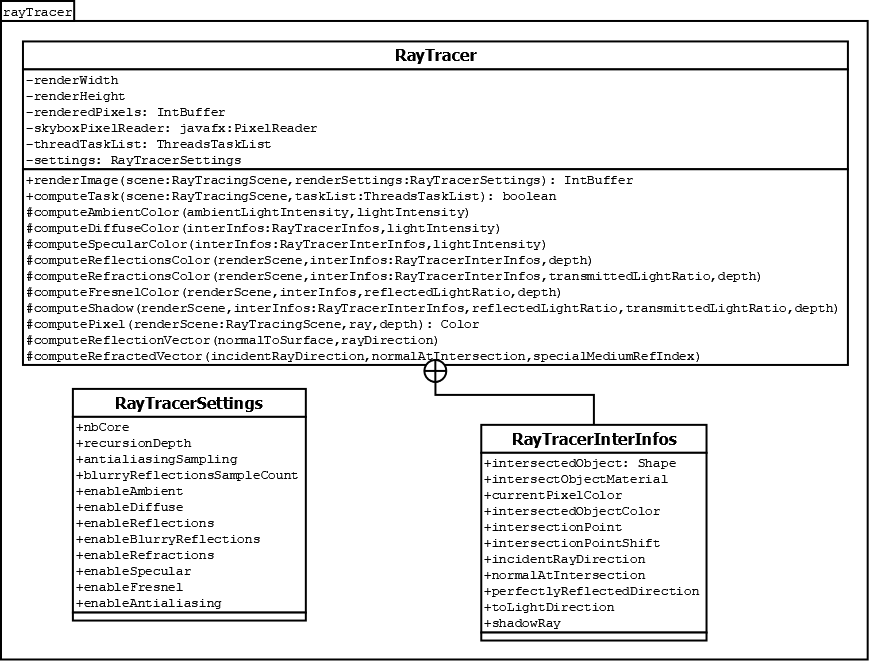
\includegraphics[width=\textwidth]{diagrammes/diagramme_RayTracer.png}}
	
	\caption{Diagramme du package RayTracer}
	\label{diagrammeRayTracer}
\end{figure}
\FloatBarrier

La classe \textit{RayTracerInterInfos} est une classe interne à RayTracer. Elle récolte toutes les informations concernant l'intersection d'un rayon et d'un objet de la scène. Cette classe permet, en interne, une gestion plus facile du ray tracer et du calcul des réflexions, réfractions, etc...

\begin{figure}[h!]
	\adjustbox{center}{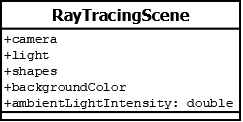
\includegraphics[width=0.52\textwidth]{diagrammes/classe_RayTracingScene.png}}
	
	\caption{Diagramme de la classe RayTracingScene contenant les informations de la scène}
	\label{diagrammeRayTracingScene}
\end{figure}
\FloatBarrier

La classe Camera, l'interface Light et la classe RayTracingScene s'organisent toutes dans le package scene:

\begin{figure}[h!]
	\adjustbox{center}{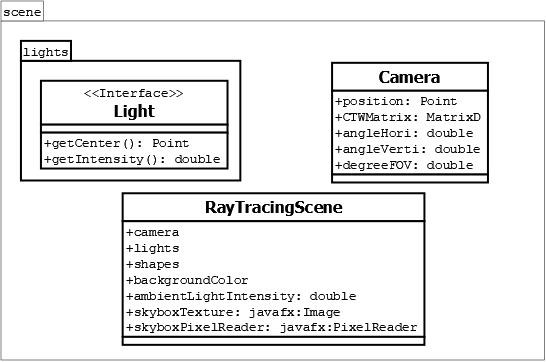
\includegraphics[width=0.75\textwidth]{diagrammes/package_scene.png}}
	
	\caption{Diagramme du package scene}
	\label{diagrammePackageScene}
\end{figure}
\FloatBarrier


\end{document}